% ==============================================================
%  AutoNexa — Critical Design Review Report  (Final Merged)
%  Sources: CDRR-2026-03-24.md · autonexa CDRR notion.txt
%           AutoNexa_CDRR_2026-03-29.tex · cdrr_perception_navigation.md
% ==============================================================
\documentclass[12pt,a4paper]{report}

% -------------------- PACKAGES --------------------
\usepackage[utf8]{inputenc}
\usepackage[T1]{fontenc}
\usepackage{lmodern}
\usepackage[a4paper,top=2.5cm,bottom=2.5cm,left=2.5cm,right=2.5cm]{geometry}
\usepackage{setspace}
\usepackage{graphicx}
\usepackage{float}
\usepackage{array}
\usepackage{booktabs}
\usepackage{longtable}
\usepackage{tabularx}
\usepackage{multirow}
\usepackage{caption}
\usepackage{subcaption}
\usepackage{titlesec}
\usepackage{fancyhdr}
\usepackage{hyperref}
\usepackage{enumitem}
\usepackage{pdflscape}
\usepackage{appendix}
\usepackage{xcolor}
\usepackage{tikz}
\usepackage{listings}
\usetikzlibrary{arrows.meta,positioning,shapes.geometric,fit,calc}

% -------------------- HYPERREF --------------------
\hypersetup{
    colorlinks=true,
    linkcolor=blue,
    urlcolor=blue,
    citecolor=blue,
    pdftitle={AutoNexa Critical Design Review Report},
    pdfauthor={AutoNexa Team},
    pdfsubject={CDRR},
    pdfkeywords={AutoNexa, CDRR, Autonomous Parking, ROS2}
}

% -------------------- LISTINGS (code/flow blocks) --------------------
\lstset{
    basicstyle=\ttfamily\small,
    breaklines=true,
    frame=single,
    backgroundcolor=\color{gray!8},
    rulecolor=\color{gray!40},
    xleftmargin=6pt,
    xrightmargin=6pt,
    aboveskip=6pt,
    belowskip=6pt
}

% -------------------- SPACING --------------------
\onehalfspacing

% -------------------- COLOURS --------------------
\definecolor{navyblue}{RGB}{26,46,74}
\definecolor{lightblue}{RGB}{220,232,245}

% -------------------- HEADER / FOOTER --------------------
\pagestyle{fancy}
\fancyhf{}
\fancyhead[L]{\textcolor{navyblue}{\textbf{AutoNexa}}}
\fancyhead[R]{\textcolor{navyblue}{Critical Design Review Report}}
\fancyfoot[C]{\thepage}
\renewcommand{\headrulewidth}{0.4pt}

% -------------------- SECTION FORMATTING --------------------
\titleformat{\chapter}[display]
    {\bfseries\Large\color{navyblue}}
    {\chaptertitlename\ \thechapter}{10pt}{\Huge}

\titleformat{\section}
    {\bfseries\large\color{navyblue}}{\thesection}{1em}{}

\titleformat{\subsection}
    {\bfseries\normalsize}{\thesubsection}{1em}{}

\titleformat{\subsubsection}
    {\bfseries\normalsize\itshape}{\thesubsubsection}{1em}{}

% -------------------- CUSTOM COMMANDS --------------------
\newcommand{\pname}{AutoNexa}
\newcommand{\reportdate}{April 2026}
\newcommand{\courseinfo}{EE493 / EE494}
\newcommand{\ver}{Version 2.0 (Merged)}

% ==============================================================
\begin{document}

% ==================== TITLE PAGE ====================
\begin{titlepage}
    \centering
    \vspace*{1.5cm}

    {\Huge \textbf{\textcolor{navyblue}{\pname}} \par}
    \vspace{0.4cm}
    {\LARGE Intelligent Parking and Recall System \par}
    \vspace{1.5cm}

    \noindent\rule{\textwidth}{1.5pt}
    \vspace{0.4cm}

    {\Huge \textbf{Critical Design Review Report} \par}
    \vspace{0.4cm}
    \noindent\rule{\textwidth}{1.5pt}

    \vspace{1cm}
    {\Large \courseinfo \par}
    \vspace{0.3cm}
    {\large \ver \par}
    \vspace{0.3cm}
    {\large \reportdate \par}

    \vfill

    \begin{flushleft}
    \textbf{Design Studio Section:} X \\[0.4cm]
    \textbf{Supervisor:} Name Surname \\[0.4cm]
    \textbf{Presented by:} \\[0.3cm]
    \quad An\i{}l Salih \c{C}olak \\
    \quad Do\u{g}ukan Zorlu \\
    \quad Emre Mende\c{s} \\
    \quad Ismayil Ibrahimli \\
    \quad Oghuz Novruzaliyev \\
    \quad Umut Kumral \\
    \end{flushleft}

    \vfill
\end{titlepage}

% ==================== FRONT MATTER ====================
\pagenumbering{roman}
\tableofcontents
\clearpage
\listoffigures
\clearpage
\listoftables
\clearpage
\pagenumbering{arabic}

% ==================== EXECUTIVE SUMMARY ====================
\chapter*{Executive Summary}
\addcontentsline{toc}{chapter}{Executive Summary}

\pname{} is a small-scale autonomous parking and recall system designed for structured indoor environments. The project goal is to develop a vehicle that can understand its surroundings, navigate safely, detect obstacles, and complete parking tasks with good positional accuracy. The system is built around a Raspberry Pi~5 running ROS~2 Jazzy for high-level autonomy, a Raspberry Pi Pico for deterministic low-level actuation, and a SLAMTEC C1 LiDAR as the primary sensing device.

Since the conceptual design stage, the project has advanced through subsystem-level testing and full prototype integration. LiDAR-based localization and navigation were validated separately before being merged into a unified live-SLAM pipeline. Motor control, power endurance, and communication integrity were also tested in isolation. These activities confirmed that individual subsystems perform acceptably and can be integrated without fundamental conflicts.

As of \reportdate, the core architecture is estimated at \textbf{80--85\% design maturity}. The safety-critical modules --- command conditioning, timeout logic, heartbeat supervision, and duplicate publisher protection --- are \textbf{100\% design-frozen} and under integration testing. The command pipeline (\texttt{/cmd\_vel} $\rightarrow$ \texttt{/cmd\_vel\_smoothed} $\rightarrow$ \texttt{/cmd\_vel\_safe} $\rightarrow$ \texttt{/pico/control\_cmd}) is fully implemented. Remaining work targets physical closed-loop trials, control-source arbitration, IMU-assisted odometry fusion, and long-duration endurance testing.

This report presents the current design status, subsystem details, test results, and the path forward to final demonstration.

% ==================== CHAPTER 1: INTRODUCTION ====================
\chapter{Introduction}

\section{Project Overview}

\pname{} is a small-scale autonomous vehicle platform for structured indoor parking scenarios. It uses LiDAR to map its environment, estimates its position through SLAM and scan matching, plans collision-aware paths to parking targets, and executes safe low-speed maneuvers through a safety-filtered software bridge to embedded actuators. The system supports both autonomous operation (goal-based navigation via RViz or a mobile app) and manual teleoperation.

\section{Current Status of the Project}

The project has moved beyond first feasibility studies. The following items are complete:

\begin{itemize}
    \item Live SLAM + Nav2 navigation baseline.
    \item Pico bridge hardening (rate limiting, acceleration capping, timeout, duplicate publisher guard).
    \item Diagnostic scripts for topic integrity, TF tree health, and control-chain validation.
    \item Rosbag recording tooling for standardized trace collection.
    \item EKF scaffolding (no IMU yet) prepared for future sensor fusion.
\end{itemize}

The following items are partially complete or in progress:

\begin{itemize}
    \item Physical E-STOP characterization under actual motion.
    \item End-to-end autonomous parking repetitions in a real test environment.
    \item Mode arbitration between Nav2 autonomous and mobile/manual control.
    \item IMU integration and EKF activation.
\end{itemize}

\section{Scope and Organization of the Report}

Chapter~2 presents the top-down system design and overall data flow. Chapters~3--5 provide detailed descriptions of the Embedded, Perception, and Navigation subsystems respectively. Chapter~6 covers test procedures and results. Chapter~7 analyzes system robustness against failure modes. Chapter~8 addresses cost, power, and schedule. Chapter~9 concludes with readiness assessment and next steps.

\section{System Operation Overview}

The \pname{} system can be understood as a continuous pipeline that runs while the vehicle is active. At each step, a clearly defined subsystem is responsible for one aspect of autonomous behavior.

\begin{enumerate}[label=\textbf{Step \arabic*:}, leftmargin=2.5cm]
    \item \textbf{Sensing.} The LiDAR sensor continuously scans the environment, producing distance data at $\sim$10~Hz over 360°. This raw data is filtered and published as \texttt{/scan}.
    \item \textbf{Localization and Mapping.} SLAM Toolbox builds a live occupancy map (\texttt{/map}) and the laser scan matcher estimates the robot's pose incrementally via ICP. Together they answer: \textit{Where am I?} and \textit{What is around me?}
    \item \textbf{Decision-Making.} Nav2 uses the current map, the robot's pose, and a target goal to compute a global path and local velocity commands (\texttt{/cmd\_vel}).
    \item \textbf{Command Conditioning.} Velocity smoothing shapes the acceleration profile, and the collision monitor checks for predicted obstacles. The output is \texttt{/cmd\_vel\_safe}.
    \item \textbf{Bridge and Final Safety.} The \texttt{cmd\_vel\_to\_pico\_bridge} applies hard velocity clamping, per-cycle acceleration limiting, timeout-to-zero, and duplicate publisher protection before publishing \texttt{/pico/control\_cmd}.
    \item \textbf{Actuation.} Pico firmware receives the bounded command, applies Ackermann inverse kinematics, and drives the steering servo and rear motors. Hardware-level safety (watchdog, E-STOP) is enforced independently at this stage.
\end{enumerate}

\noindent In summary: \textbf{sensing $\rightarrow$ localization $\rightarrow$ planning $\rightarrow$ command conditioning $\rightarrow$ actuation}.

% ==================== CHAPTER 2: SYSTEM DESIGN ====================
\chapter{System Design}

\section{Overall System Description}

The architecture is a strictly layered perception-to-actuation chain with no direct coupling between high-level planning and hardware. LiDAR data drives both mapping and odometry. Nav2 produces motion requests that are never sent directly to the motors; they must pass through two software safety stages and a bridge layer before reaching the Pico. The Pico itself applies a final hardware-level watchdog independently of the RPi5 software.

\section{System-Level Block Diagram}

\begin{figure}[H]
\centering
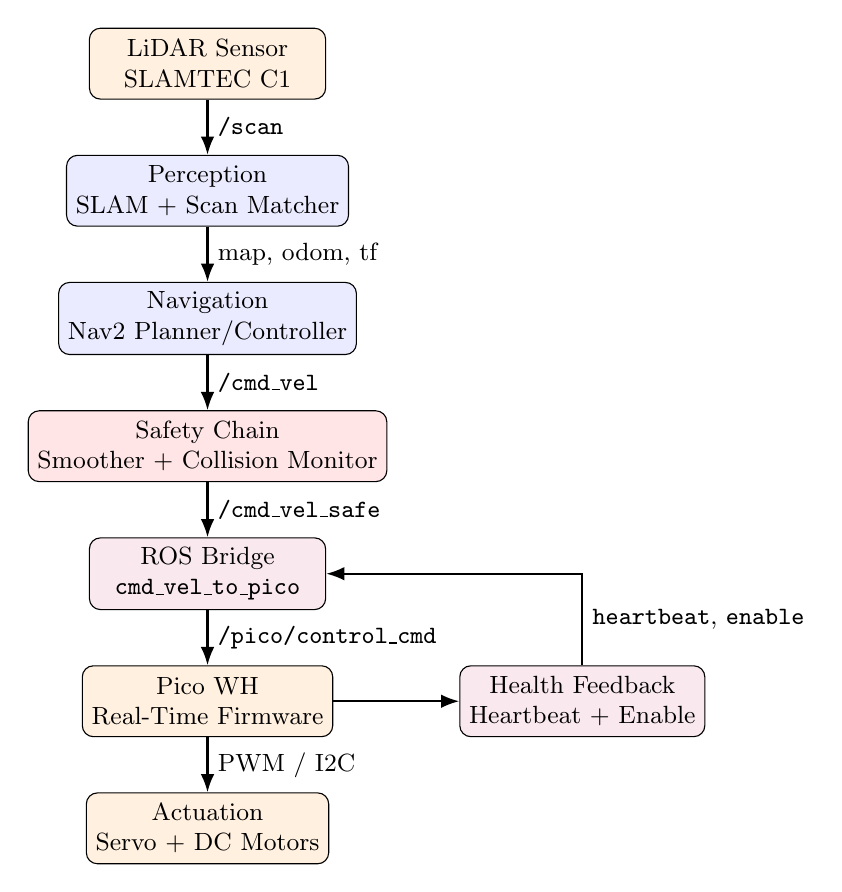
\begin{tikzpicture}[
    node distance=7mm and 16mm,
    block/.style={draw, rounded corners, minimum width=3cm, minimum height=0.9cm,
                  align=center, fill=blue!8, font=\small},
    safety/.style={draw, rounded corners, minimum width=3cm, minimum height=0.9cm,
                   align=center, fill=red!10, font=\small},
    hw/.style={draw, rounded corners, minimum width=3cm, minimum height=0.9cm,
               align=center, fill=orange!12, font=\small},
    io/.style={draw, rounded corners, minimum width=3cm, minimum height=0.9cm,
               align=center, fill=purple!9, font=\small},
    line/.style={-Latex, thick}
]
\node[hw]      (lidar)      {LiDAR Sensor\\SLAMTEC C1};
\node[block,   below=of lidar]   (percep)  {Perception\\SLAM + Scan Matcher};
\node[block,   below=of percep]  (nav2)    {Navigation\\Nav2 Planner/Controller};
\node[safety,  below=of nav2]    (safety)  {Safety Chain\\Smoother + Collision Monitor};
\node[io,      below=of safety]  (bridge)  {ROS Bridge\\\texttt{cmd\_vel\_to\_pico}};
\node[hw,      below=of bridge]  (pico)    {Pico WH\\Real-Time Firmware};
\node[hw,      below=of pico]    (act)     {Actuation\\Servo + DC Motors};
\node[io,      right=of pico]    (health)  {Health Feedback\\Heartbeat + Enable};

\draw[line] (lidar)  -- node[right,font=\small]{\texttt{/scan}}        (percep);
\draw[line] (percep) -- node[right,font=\small]{map, odom, tf}          (nav2);
\draw[line] (nav2)   -- node[right,font=\small]{\texttt{/cmd\_vel}}    (safety);
\draw[line] (safety) -- node[right,font=\small]{\texttt{/cmd\_vel\_safe}} (bridge);
\draw[line] (bridge) -- node[right,font=\small]{\texttt{/pico/control\_cmd}} (pico);
\draw[line] (pico)   -- node[right,font=\small]{PWM / I2C}             (act);
\draw[line] (pico.east)   -- (health.west);
\draw[line] (health.north) |- node[pos=0.25,right,font=\small]
            {\texttt{heartbeat}, \texttt{enable}} (bridge.east);
\end{tikzpicture}
\caption{System-level block diagram of the \pname{} platform.}
\label{fig:system_block}
\end{figure}

\section{Main Data and Control Signals}

\begin{table}[H]
\centering
\caption{Key ROS2 topics and their roles in the system.}
\label{tab:signals}
\begin{tabularx}{\textwidth}{|p{3.2cm}|p{2.2cm}|p{2.8cm}|X|}
\hline
\textbf{Topic} & \textbf{Type} & \textbf{Source $\rightarrow$ Sink} & \textbf{Purpose} \\
\hline
\texttt{/scan} & \texttt{LaserScan} & LiDAR $\rightarrow$ SLAM, Nav2 & Raw and filtered environment sensing \\
\hline
\texttt{/map} & \texttt{OccupancyGrid} & SLAM Toolbox $\rightarrow$ Nav2 & Live occupancy map \\
\hline
\texttt{/odom} & \texttt{Odometry} & Scan matcher $\rightarrow$ Nav2 & Incremental pose estimate \\
\hline
\texttt{/cmd\_vel} & \texttt{Twist} & Nav2 $\rightarrow$ smoother & Raw motion command \\
\hline
\texttt{/cmd\_vel\_safe} & \texttt{Twist} & Collision monitor $\rightarrow$ bridge & Safety-filtered command \\
\hline
\texttt{/pico/control\_cmd} & \texttt{TwistStamped} & Bridge $\rightarrow$ Pico & Bounded velocity command to MCU \\
\hline
\texttt{/pico/enable} & \texttt{Bool} & Bridge $\rightarrow$ Pico & Motor enable/disable \\
\hline
\texttt{/pico/heartbeat} & \texttt{Bool} & Bridge $\rightarrow$ Pico & Liveness check (200 ms timeout) \\
\hline
\texttt{/pico/odom} & \texttt{Odometry} & Pico $\rightarrow$ RPi5 & Wheel-encoder odometry \\
\hline
\texttt{/tf}, \texttt{/tf\_static} & TF transforms & Multiple nodes & Frame consistency \\
\hline
\end{tabularx}
\end{table}

\section{System and Subsystem Requirements}

\subsection{System-Level Requirements}

\begin{table}[H]
\centering
\caption{System-level requirements.}
\label{tab:sys_req}
\begin{tabularx}{\textwidth}{|p{1.7cm}|X|p{3cm}|}
\hline
\textbf{ID} & \textbf{Requirement} & \textbf{Target} \\
\hline
SYS-01 & Autonomous navigation in a constrained indoor parking environment & Functional completion \\
\hline
SYS-02 & Safe low-speed operation & $\leq$ 0.5 m/s; $\sim$0.1 m/s for final approach \\
\hline
SYS-03 & Precise autonomous parking & Final position error $\leq \pm$5 cm \\
\hline
SYS-04 & Summon / recall operation & Return to user-defined location on command \\
\hline
SYS-05 & Collision-aware command output & No unsafe direct path from planner to actuators \\
\hline
SYS-06 & Safe stop on command loss & Timeout $\leq$ 200 ms \\
\hline
SYS-07 & Deterministic command update & 30 Hz nominal bridge publish rate \\
\hline
SYS-08 & Obstacle detection & Static and dynamic obstacles $\geq$ 5 cm diameter \\
\hline
SYS-09 & Wireless user interaction & Mobile app control at $\geq$ 3 m range \\
\hline
SYS-10 & Power endurance & All subsystems operational for $\geq$ 15 min \\
\hline
\end{tabularx}
\end{table}

\subsection{Subsystem Requirements}

\begin{table}[H]
\centering
\caption{Localization subsystem requirements.}
\label{tab:loc_req}
\begin{tabularx}{\textwidth}{|p{4cm}|X|}
\hline
\textbf{Requirement} & \textbf{Description} \\
\hline
Scan precision & Resolve geometric features with minimum resolution of 2 cm. \\
\hline
Update frequency & Localization estimate updated at $\geq$ 10 Hz. \\
\hline
Blind spot minimization & Detect obstacles as close as 0.05 m. \\
\hline
Map consistency & Map remains consistent after repeated passes and loop closure. \\
\hline
Stable pose estimation & Provide stable, repeatable pose for navigation during low-speed operation. \\
\hline
\end{tabularx}
\end{table}

\begin{table}[H]
\centering
\caption{Navigation subsystem requirements.}
\label{tab:nav_req}
\begin{tabularx}{\textwidth}{|p{4cm}|X|}
\hline
\textbf{Requirement} & \textbf{Description} \\
\hline
Goal-based path generation & Generate a path after a valid parking or recall target is defined. \\
\hline
Collision-free planning & Produce collision-free paths on the current map. \\
\hline
Real-time operation & Update path information without blocking localization. \\
\hline
Navigation accuracy & Guide vehicle to target with acceptable final distance error. \\
\hline
Narrow-space robustness & Remain functional in constrained indoor paths. \\
\hline
\end{tabularx}
\end{table}

\begin{table}[H]
\centering
\caption{Control subsystem requirements.}
\label{tab:ctrl_req}
\begin{tabularx}{\textwidth}{|p{4cm}|X|}
\hline
\textbf{Requirement} & \textbf{Description} \\
\hline
Ackermann motion model & Convert body velocity commands to steering angle and differential wheel speeds. \\
\hline
Command rate & Execute control commands at $\geq$ 30 Hz. \\
\hline
Safety timeout & Stop all motors within 200 ms of communication loss. \\
\hline
Emergency stop & Latch E-STOP state until explicitly cleared; independent of software stack. \\
\hline
Velocity saturation & Enforce maximum velocity and acceleration limits before actuation. \\
\hline
\end{tabularx}
\end{table}

\section{Design Modifications Since Conceptual Design Report}

\subsection{Modification 1 --- Architecture Shift to Live SLAM}
\textbf{Original:} static-map-dominant workflow.\\
\textbf{Issue:} lower robustness during iterative development and mapping updates.\\
\textbf{Change:} live SLAM + Nav2 baseline adopted as the primary and only operational mode.\\
\textbf{Justification:} eliminates map-reload overhead, improves continuous integration observability.

\subsection{Modification 2 --- Safety Chain Hardening}
\textbf{Original:} basic bridge forwarding with no duplicate-source protection.\\
\textbf{Issue:} potential unsafe behavior when multiple publishers exist or a command source disappears.\\
\textbf{Change:} file-based lock, ROS graph duplicate-publisher monitoring, timeout-to-zero, and safe self-termination.\\
\textbf{Justification:} contains control conflicts; safer degraded behavior with no code change required at the Nav2 level.

\subsection{Modification 3 --- Battery Selection}
\textbf{Original:} lithium-ion battery with BMS.\\
\textbf{Issue:} current fluctuations on the 5 V logic rail caused RPi5 display instability.\\
\textbf{Change:} switched to 12.8 V, 7 Ah lead-acid battery.\\
\textbf{Justification:} more stable voltage output under transient motor loads; lower cost.

\section{Compatibility Analysis of Subsystems}

\begin{table}[H]
\centering
\caption{Interface compatibility summary.}
\label{tab:compat}
\begin{tabularx}{\textwidth}{|p{2.8cm}|p{2.8cm}|p{2.4cm}|X|}
\hline
\textbf{Source} & \textbf{Destination} & \textbf{Interface} & \textbf{Notes} \\
\hline
Raspberry Pi 5 & Pico WH & USB CDC / micro-ROS & High-level command and telemetry exchange at 115,200 baud \\
\hline
Pico WH & Motor driver & I2C, 100 kHz & Speed commands and encoder reads via Hiwonder protocol \\
\hline
Pico WH & Steering servo & PWM, 50 Hz & Angle-to-pulse linear mapping; GPIO 12 \\
\hline
LiDAR & Raspberry Pi 5 & USB/UART, 460,800 baud & Range scan for SLAM and costmaps \\
\hline
Encoders & Pico WH & I2C read & Wheel velocity for odometry integration \\
\hline
\end{tabularx}
\end{table}

\begin{table}[H]
\centering
\caption{Interface risks and mitigations.}
\label{tab:risks}
\begin{tabularx}{\textwidth}{|p{3.5cm}|X|X|}
\hline
\textbf{Risk} & \textbf{Impact} & \textbf{Mitigation} \\
\hline
Multiple publishers on \texttt{/pico/*} & Conflicting commands to Pico & Lock file + ROS graph duplicate-publisher watchdog \\
\hline
Stale process on serial port & LiDAR data loss on relaunch & Preflight kill check + by-id serial path discipline \\
\hline
Missing IMU & Odometry drift during dynamic maneuvers & Keep EKF optional; stage integration when IMU arrives \\
\hline
Manual / auto command conflict & Control instability & Introduce explicit AUTO / MANUAL / ESTOP arbitration policy \\
\hline
\end{tabularx}
\end{table}

% ==================== CHAPTER 3: EMBEDDED SUBSYSTEM ====================
\chapter{Embedded Subsystem}

\section{Overview}

The embedded subsystem runs on a Raspberry Pi Pico (RP2040, ARM Cortex-M0+) and sits at the bottom of the software stack. Its job is to translate velocity commands from ROS2 into physical actuator outputs and to enforce hardware-level safety independently of anything running on the Raspberry Pi 5.

The firmware is written in C using the Pico SDK with no RTOS. A single 50 Hz hardware-timer loop is the only scheduling primitive. The build system produces two targets:

\begin{table}[H]
\centering
\caption{Pico firmware build targets.}
\label{tab:pico_builds}
\begin{tabularx}{\textwidth}{|p{4.5cm}|X|}
\hline
\textbf{Target} & \textbf{Purpose} \\
\hline
\texttt{autonexa\_pico} & ASCII serial CLI --- bench testing and hardware validation without ROS2 \\
\hline
\texttt{autonexa\_pico\_uros} & micro-ROS production mode --- receives commands as ROS2 topics over USB serial \\
\hline
\end{tabularx}
\end{table}

\section{Hardware Interfaces}

\begin{table}[H]
\centering
\caption{Pico hardware interface summary.}
\label{tab:pico_hw}
\begin{tabularx}{\textwidth}{|p{2.8cm}|p{2cm}|p{2.8cm}|X|}
\hline
\textbf{Interface} & \textbf{Protocol} & \textbf{Connection} & \textbf{Device} \\
\hline
Steering servo & PWM, 50 Hz & GPIO 12 & LD-1501MG ($\pm$30\textdegree{}, 500--2500 $\mu$s) \\
\hline
Motor driver & I2C0, 100 kHz & SDA=GPIO0, SCL=GPIO1 & Hiwonder YX-4055AM (addr \texttt{0x34}) \\
\hline
Left rear motor & --- & Driver ch.\ M2 & JGB37-520R30, 12 V DC \\
\hline
Right rear motor & --- & Driver ch.\ M4 & JGB37-520R30, 12 V DC \\
\hline
Host communications & USB CDC & --- & Raspberry Pi 5 at 115,200 baud \\
\hline
Heartbeat LED & GPIO output & GPIO 25 & On-board LED \\
\hline
\end{tabularx}
\end{table}

\section{Vehicle Parameters}

All physical constants are defined in \texttt{pico\_firmware/include/config.h}.

\begin{table}[H]
\centering
\caption{Vehicle physical and control parameters.}
\label{tab:vehicle_params}
\begin{tabularx}{\textwidth}{|p{4.5cm}|p{3cm}|X|}
\hline
\textbf{Parameter} & \textbf{Value} & \textbf{Notes} \\
\hline
Wheelbase & 0.25 m & Front-to-rear axle distance \\
\hline
Track width & 0.20 m & Left-to-right wheel centreline \\
\hline
Wheel radius & 0.033 m & 66 mm diameter \\
\hline
Max steering angle & $\pm$30\textdegree{} ($\pm$0.5236 rad) & Hardware limit of servo linkage \\
\hline
Motor gear ratio & 1:30 & JGB37-520R30, 12 V DC \\
\hline
Encoder edges per wheel rev & 1320 & 11 $\times$ 4 $\times$ 30 \\
\hline
Control loop rate & 50 Hz (20 ms) & Hardware timer driven \\
\hline
Command timeout & 200 ms & Watchdog threshold \\
\hline
\end{tabularx}
\end{table}

\section{Control Loop}

The 50 Hz loop executes the following sequence every 20 ms:

\begin{lstlisting}
[50 Hz timer tick]
  |
  v
1. Read encoders       -- I2C from Hiwonder driver
  |
  v
2. Forward kinematics  -- delta ticks -> wheel velocities -> integrate odom (x, y, yaw)
  |
  v
3. Safety check        -- increment timeout counter, check E-STOP, update LED
  |
  v
4. Apply actuators     -- gated by safety_is_ok()
   - Steering angle -> servo PWM
   - Wheel speeds   -> I2C motor driver
  |
  v
5a. micro-ROS mode:              | 5b. Serial CLI mode:
    spin subscribers             |     parse incoming command
    publish /pico/odom  @ 20 Hz  |     print telemetry @ 10 Hz
    publish /pico/joints@ 10 Hz  |
\end{lstlisting}

\section{Ackermann Kinematics}

ROS2 sends body-frame velocity commands $(v_x, \omega_z)$. The firmware implements both directions of the Ackermann model.

\textbf{Inverse kinematics} (command $\rightarrow$ actuators): computes steering angle $\delta = \arctan(L \cdot \omega_z / v_x)$ and left/right differential wheel speeds using the turning radius $R = L / \tan(\delta)$. Straight-line motion is handled as the degenerate case where both wheel speeds equal $v_x$.

\textbf{Forward kinematics} (encoders $\rightarrow$ odometry): integrates encoder ticks each 20 ms cycle into an $(x, y, \psi)$ pose estimate using the bicycle model:
$\bar{v} = (v_L + v_R)/2$, $\dot{\psi} = \bar{v} \tan(\delta)/L$, then numerically integrating position. This is published on \texttt{/pico/odom} at 20 Hz.

The Pico odometry is currently not consumed by Nav2 --- the RPi5 uses the laser scan matcher as the primary odometry source. It will become an active input once the EKF is activated.

\section{Safety System}

All actuator writes are gated through \texttt{safety\_is\_ok()}. Two independent conditions can block actuation:

\begin{table}[H]
\centering
\caption{Embedded safety states and behaviors.}
\label{tab:pico_safety}
\begin{tabularx}{\textwidth}{|p{2.2cm}|p{2.5cm}|p{1.8cm}|p{2.5cm}|X|}
\hline
\textbf{State} & \textbf{Cause} & \textbf{Motors} & \textbf{LED} & \textbf{Recovery} \\
\hline
Normal & --- & Running & 1 Hz blink & --- \\
\hline
Timed out & No command for 200 ms & Stopped + centred & 1 Hz blink & Next valid command \\
\hline
E-STOP & Explicit trigger & Stopped + centred & 5 Hz blink & Explicit clear only \\
\hline
\end{tabularx}
\end{table}

The E-STOP is a latching flag; it does not self-recover. This is intentional --- an E-STOP triggered during motion should require deliberate human action to clear.

\section{micro-ROS Topics}

In production mode, the Pico runs as a micro-ROS node (\texttt{pico\_controller}, domain 0) over XRCE-DDS on USB serial. On boot it blocks in a ping loop until the RPi5 micro-ROS agent responds before starting the control loop.

\begin{table}[H]
\centering
\caption{micro-ROS topics published and subscribed by the Pico.}
\label{tab:uros_topics}
\begin{tabularx}{\textwidth}{|p{3.8cm}|p{1.6cm}|p{3.2cm}|p{1.3cm}|X|}
\hline
\textbf{Topic} & \textbf{Direction} & \textbf{Type} & \textbf{Rate} & \textbf{Description} \\
\hline
\texttt{/pico/control\_cmd} & RPi5$\rightarrow$Pico & \texttt{TwistStamped} & 30 Hz & $v_x$, $\omega_z$ velocity command \\
\hline
\texttt{/pico/enable} & RPi5$\rightarrow$Pico & \texttt{Bool} & 30 Hz & Motor enable/disable \\
\hline
\texttt{/pico/heartbeat} & RPi5$\rightarrow$Pico & \texttt{Bool} & 5 Hz & Liveness; timeout = 200 ms \\
\hline
\texttt{/pico/odom} & Pico$\rightarrow$RPi5 & \texttt{Odometry} & 20 Hz & Wheel-encoder pose estimate \\
\hline
\texttt{/pico/joint\_feedback} & Pico$\rightarrow$RPi5 & \texttt{JointState} & 10 Hz & Wheel velocities + steering angle \\
\hline
\texttt{/pico/estop} (srv) & RPi5$\rightarrow$Pico & \texttt{SetBool} & On demand & Activate or clear E-STOP \\
\hline
\end{tabularx}
\end{table}

\section{Known Limitations and Open Items}

\begin{table}[H]
\centering
\caption{Embedded subsystem open items.}
\label{tab:pico_limits}
\begin{tabularx}{\textwidth}{|p{3.8cm}|p{1.4cm}|X|}
\hline
\textbf{Item} & \textbf{Severity} & \textbf{Resolution Path} \\
\hline
Pico odometry not yet fused into TF chain & Medium & Will be integrated as EKF input when IMU is connected \\
\hline
USB CDC sync loss on long sessions & Low & Pico watchdog catches it and stops motors; agent relaunch required to recover \\
\hline
No motor stall / overcurrent detection & Low & Hardware addition needed; out of current scope \\
\hline
\end{tabularx}
\end{table}

% ==================== CHAPTER 4: PERCEPTION SUBSYSTEM ====================
\chapter{Perception Subsystem}

\section{Overview}

The perception subsystem builds a real-time geometric model of the environment and produces the pose estimate that everything downstream depends on. The system uses a \textbf{LiDAR-first architecture}: the 2D rotating LiDAR is the sole source of both mapping (SLAM Toolbox) and incremental dead-reckoning (laser scan matching). The design supports two operational modes:

\begin{table}[H]
\centering
\caption{Perception operational modes.}
\label{tab:perc_modes}
\begin{tabularx}{\textwidth}{|p{1.5cm}|p{2.8cm}|p{2.8cm}|p{2.2cm}|X|}
\hline
\textbf{Mode} & \textbf{Active Sensors} & \textbf{Odometry Source} & \textbf{Map Source} & \textbf{Status} \\
\hline
A & SLAMTEC C1 only & laser\_scan\_matcher & SLAM Toolbox & \textbf{Active} (current default) \\
\hline
B & SLAMTEC C1 + IMX219 camera & EKF (LiDAR + IMU) & SLAM Toolbox & Planned --- URDF and mobile app ready; ROS2 node pending \\
\hline
\end{tabularx}
\end{table}

Switching between modes will be a launch argument, not a code change. In Mode B, the camera feeds the goal-setting logic for ArUco-guided parking approach; it does not affect the SLAM or TF chain.

\section{SLAMTEC C1 LiDAR}

\begin{table}[H]
\centering
\caption{SLAMTEC C1 LiDAR specifications and ROS2 integration.}
\label{tab:lidar_specs}
\begin{tabularx}{\textwidth}{|p{4cm}|X|}
\hline
\textbf{Property} & \textbf{Value} \\
\hline
Measurement principle & ToF / triangulation (rotating 2D) \\
\hline
Field of view & 360\textdegree{} \\
\hline
Operational range (configured) & 0.05 m -- 4.0 m \\
\hline
Scan frequency & $\sim$10 Hz \\
\hline
ROS2 driver & \texttt{sllidar\_ros2} \\
\hline
Published topic & \texttt{/scan} (\texttt{sensor\_msgs/LaserScan}) \\
\hline
Frame ID & \texttt{laser\_link} \\
\hline
Serial interface & USB CDC at 460,800 baud \\
\hline
Physical mounting & +150 mm fwd, +120 mm above \texttt{base\_link} \\
\hline
\end{tabularx}
\end{table}

\textbf{Known failure mode.} If \texttt{sllidar\_node} is killed without a clean shutdown, the OS may not release the file descriptor on \texttt{/dev/ttyUSB0}. The next launch then gets an \texttt{SL\_RESULT\_OPERATION\_TIMEOUT}. The fix is to kill stale processes and use the stable \texttt{/dev/serial/by-id/} path, which is deterministic across USB re-enumerations.

\section{Scan Filter Chain}

Raw \texttt{/scan} passes through a four-stage \texttt{laser\_filters} chain before being consumed by SLAM or costmaps.

\begin{table}[H]
\centering
\caption{Laser scan filter chain stages.}
\label{tab:filters}
\begin{tabularx}{\textwidth}{|p{0.5cm}|p{3.5cm}|p{3cm}|X|}
\hline
\textbf{\#} & \textbf{Filter Type} & \textbf{Key Parameters} & \textbf{Purpose} \\
\hline
1 & \texttt{LaserScanRangeFilter} & min: 0.05 m, max: 4.0 m & Remove out-of-range returns that confuse SLAM \\
\hline
2 & \texttt{ScanShadowsFilter} & angle: 10\textdegree--170\textdegree{}, neighbors: 20 & Remove grazing-angle ghost points on object edges \\
\hline
3 & \texttt{MedianFilter} & observations: 5, queue: 10 & Suppress flicker on reflective or glass surfaces \\
\hline
4 & \texttt{LaserScanOutlierFilter} & threshold: 0.5 m, window: 5 & Remove isolated spikes from multi-path reflections \\
\hline
\end{tabularx}
\end{table}

\section{Laser Scan Matcher --- Odometry}

All incremental dead-reckoning is performed by ICP scan-to-scan matching (\texttt{ros2\_laser\_scan\_matcher}). It publishes \texttt{/odom} and the \texttt{odom$\rightarrow$base\_link} TF transform.

\begin{table}[H]
\centering
\caption{Laser scan matcher configuration.}
\label{tab:scan_matcher}
\begin{tabularx}{\textwidth}{|p{4.5cm}|p{2cm}|X|}
\hline
\textbf{Parameter} & \textbf{Value} & \textbf{Meaning} \\
\hline
Keyframe distance threshold & 0.10 m & New keyframe after 10 cm of motion \\
\hline
Keyframe angle threshold & 10\textdegree{} & New keyframe after 10\textdegree{} of rotation \\
\hline
ICP max iterations & 30 & Convergence cap per scan \\
\hline
Max correspondence distance & 0.30 m & Points further apart are not matched \\
\hline
Max angular correction & 45\textdegree{} & Guards against catastrophic misalignment \\
\hline
\end{tabularx}
\end{table}

Covariance is computed from the ICP residual and included in the Odometry message. Scan matching accumulates drift over time; this is the primary motivation for IMU fusion. For short parking maneuvers (a few meters), drift is negligible.

\section{SLAM Toolbox --- Live Mapping}

SLAM Toolbox runs in asynchronous mapping mode (\texttt{async\_slam\_toolbox\_node}). There is no pre-loaded map; the occupancy grid grows as the robot explores.

\begin{table}[H]
\centering
\caption{SLAM Toolbox configuration parameters.}
\label{tab:slam}
\begin{tabularx}{\textwidth}{|p{4cm}|p{2.2cm}|X|}
\hline
\textbf{Parameter} & \textbf{Value} & \textbf{Notes} \\
\hline
Map resolution & 0.02 m/pixel & 2 cm chosen for parking precision; a 0.5 m $\times$ 1 m slot = 25$\times$50 cells \\
\hline
Update distance & 0.05 m & Map updated after 5 cm of motion \\
\hline
Update heading & 0.05 rad ($\sim$3\textdegree{}) & Map updated on small rotations \\
\hline
Fallback update interval & 1.0 s & Update even when stationary \\
\hline
Loop closure search radius & 3.0 m & Candidates within 3 m are evaluated \\
\hline
Provide odometry frame & \texttt{false} & scan\_matcher owns \texttt{odom$\rightarrow$base\_link} \\
\hline
\end{tabularx}
\end{table}

\section{TF Tree}

\begin{lstlisting}
map
 |  <-- SLAM Toolbox (map-level correction; updated as map refines)
 v
odom
 |  <-- laser_scan_matcher (incremental dead-reckoning, ~10 Hz)
 v
base_link
 |  <-- static_transform_publisher (fixed sensor placement)
 v
laser_link
\end{lstlisting}

The split between \texttt{map$\rightarrow$odom} and \texttt{odom$\rightarrow$base\_link} follows the ROS2 convention: the latter never jumps, guaranteeing smooth velocity commands. SLAM Toolbox adjusts \texttt{map$\rightarrow$odom} to keep the global pose consistent. When the EKF is activated, \texttt{robot\_localization} will take over \texttt{odom$\rightarrow$base\_link} using fused LiDAR + IMU data.

\section{Planned Extensions}

\textbf{IMU Fusion.} The EKF skeleton (\texttt{ekf\_fusion.launch.py}, \texttt{ekf\_2d\_no\_imu.yaml}) is already in the repository. Once an IMU is connected, the plan is to feed \texttt{/imu/data} and \texttt{/odom} into \texttt{robot\_localization}, enable TF publishing, and point Nav2 at \texttt{/odometry/filtered}. This significantly reduces drift during sharp turns.

\textbf{Camera Integration (Mode B).} The IMX219 camera link is defined in the URDF. The Flutter mobile app decodes ArUco markers and sends their poses via HTTP. The remaining work is a ROS2 image publisher node and a parking coordinator that refines the Nav2 goal using the live marker pose for the final 0.5 m approach.

\section{Known Limitations}

\begin{table}[H]
\centering
\caption{Perception subsystem open items.}
\label{tab:perc_limits}
\begin{tabularx}{\textwidth}{|p{3.5cm}|p{1.4cm}|X|}
\hline
\textbf{Item} & \textbf{Severity} & \textbf{Resolution Path} \\
\hline
Scan-only odometry drift on long runs & Medium & Resolved by IMU EKF fusion \\
\hline
LiDAR serial port lock on hard kill & Medium & Use by-id path; add preflight process check \\
\hline
ICP diverges in featureless corridors & Low & Limit angular velocity; long-term: IMU bridges featureless segments \\
\hline
Camera not yet integrated & Low & URDF and mobile app ready; ROS2 node pending \\
\hline
\end{tabularx}
\end{table}

% ==================== CHAPTER 5: NAVIGATION SUBSYSTEM ====================
\chapter{Navigation Subsystem}

\section{Overview}

The navigation subsystem takes a goal pose --- from RViz or the mobile app --- and produces velocity commands that move the robot to that goal while avoiding obstacles. It uses the ROS~2 Nav2 stack on top of the live SLAM map. There is no static map and no separate localization phase; navigation requests can be sent as soon as the TF tree is healthy.

\section{Global Planner --- NavfnPlanner}

NavfnPlanner performs wavefront A* over the global costmap (live SLAM map + obstacle layer).

\begin{table}[H]
\centering
\caption{Global planner parameters.}
\label{tab:planner}
\begin{tabularx}{\textwidth}{|p{4cm}|p{2cm}|X|}
\hline
\textbf{Parameter} & \textbf{Value} & \textbf{Notes} \\
\hline
Plugin & NavfnPlanner & Standard Nav2 A* \\
\hline
Goal tolerance & 0.05 m & \\
\hline
Allow unknown cells & \texttt{false} & Robot will not plan into unmapped space \\
\hline
Output & \texttt{/plan} & \texttt{nav\_msgs/Path} \\
\hline
\end{tabularx}
\end{table}

Because \texttt{allow\_unknown} is false, the operator should perform a slow drive-through to populate the map before sending a parking goal.

\section{Local Controller --- DWB Local Planner}

DWB samples short-horizon velocity trajectories and scores each against seven critics, commanding the highest-scoring trajectory at 10 Hz.

\begin{table}[H]
\centering
\caption{DWB velocity and acceleration limits.}
\label{tab:dwb_limits}
\begin{tabularx}{\textwidth}{|p{5cm}|p{2cm}|X|}
\hline
\textbf{Parameter} & \textbf{Value} & \textbf{Notes} \\
\hline
Max forward speed & 0.30 m/s & Conservative for parking precision \\
\hline
Max reverse speed & $-$0.10 m/s & Limited reverse \\
\hline
Max yaw rate & 0.50 rad/s & $\sim$28\textdegree/s \\
\hline
Forward acceleration & 1.5 m/s$^2$ & \\
\hline
Angular acceleration & 2.0 rad/s$^2$ & \\
\hline
XY goal tolerance & 0.05 m & \\
\hline
Yaw goal tolerance & 0.10 rad ($\sim$6\textdegree{}) & \\
\hline
\end{tabularx}
\end{table}

\begin{table}[H]
\centering
\caption{DWB trajectory critics.}
\label{tab:critics}
\begin{tabularx}{\textwidth}{|p{3cm}|p{1.5cm}|X|}
\hline
\textbf{Critic} & \textbf{Weight} & \textbf{What It Penalizes} \\
\hline
PathAlign & 32.0 & Deviation from planned path direction \\
\hline
PathDist & 32.0 & Distance from trajectory end to planned path \\
\hline
RotateToGoal & 32.0 & Not aligning with goal heading when close \\
\hline
GoalAlign & 24.0 & Heading misalignment with goal pose \\
\hline
GoalDist & 24.0 & Distance from trajectory end to goal \\
\hline
BaseObstacle & 0.02 & Proximity to costmap obstacles \\
\hline
Oscillation & default & Repetitive back-and-forth motion \\
\hline
\end{tabularx}
\end{table}

\section{Costmap Configuration}

Both costmaps use 0.02 m/cell resolution, matching the SLAM map, to avoid resampling artifacts.

\begin{table}[H]
\centering
\caption{Local and global costmap parameters.}
\label{tab:costmaps}
\begin{tabularx}{\textwidth}{|p{3.5cm}|p{2.2cm}|p{2.2cm}|X|}
\hline
\textbf{Parameter} & \textbf{Local} & \textbf{Global} & \textbf{Notes} \\
\hline
Frame & \texttt{odom} & \texttt{map} & \\
\hline
Size / Coverage & 2 m $\times$ 2 m rolling & Full map extent & \\
\hline
Update frequency & 5.0 Hz & 1.0 Hz & \\
\hline
Inflation radius & 0.20 m & 0.15 m & Local is larger to account for linkage hardware \\
\hline
Layers & obstacle + inflation & static + obstacle + inflation & \\
\hline
\end{tabularx}
\end{table}

\section{Velocity Pipeline}

Between the controller and the Pico, the command passes through three conditioning stages:

\begin{lstlisting}
Controller Server   /cmd_vel (~10 Hz)
        |
        v
Velocity Smoother   /cmd_vel_smoothed (20 Hz)
  - acceleration shaping, open-loop
        |
        v
Collision Monitor   /cmd_vel_safe
  - 1.2 s forward trajectory simulation
        |
        v
cmd_vel_to_pico_bridge   /pico/control_cmd (30 Hz)
  - velocity clamping (+/-0.35 m/s, +/-0.8 rad/s)
  - per-cycle accel limit (0.8 m/s2, 1.2 rad/s2)
  - 200 ms timeout-to-zero
  - duplicate publisher guard
        |
        v
micro-ROS agent (USB, 115200 baud)
        |
        v
Pico firmware (50 Hz)  ->  Servo + Motors
\end{lstlisting}

\section{Safety Layer Stack}

\begin{table}[H]
\centering
\caption{Navigation safety layers (outermost to innermost).}
\label{tab:safety_layers}
\begin{tabularx}{\textwidth}{|p{0.5cm}|p{3cm}|p{3cm}|X|}
\hline
\textbf{\#} & \textbf{Node} & \textbf{Trigger} & \textbf{Action} \\
\hline
1 & Velocity Smoother & Any velocity change & Ramp output; prevent torque spikes \\
\hline
2 & Collision Monitor & Predicted collision within 1.2 s & Reduce or zero velocity \\
\hline
3 & Bridge: vel clamp & Command exceeds limits & Hard clip $v_x$ and $\omega_z$ \\
\hline
4 & Bridge: accel cap & Excessive inter-cycle delta & Smooth remaining step changes \\
\hline
5 & Bridge: timeout & No command for 200 ms & Ramp to zero, disable motors \\
\hline
6 & Pico watchdog & No \texttt{/pico/control\_cmd} for 200 ms & Hardware motor disable \\
\hline
7 & Pico E-STOP & E-STOP signal & Latching motor disable \\
\hline
\end{tabularx}
\end{table}

Layers 5 and 6 use the same 200 ms threshold but operate independently: layer 5 acts in RPi5 software, layer 6 acts in Pico firmware. If the USB serial link drops, layer 5 does not fire but layer 6 still does.

\section{Update Rates and End-to-End Latency}

\begin{table}[H]
\centering
\caption{Navigation pipeline update rates and latency contributions.}
\label{tab:latency}
\begin{tabularx}{\textwidth}{|p{4.5cm}|p{2cm}|X|}
\hline
\textbf{Stage} & \textbf{Rate} & \textbf{Typical Latency} \\
\hline
LiDAR scan & $\sim$10 Hz & $<$100 ms \\
\hline
Scan filter chain & Inline & 20--30 ms \\
\hline
Laser scan matcher & Per keyframe & 20--50 ms \\
\hline
SLAM Toolbox map update & 1.0 Hz & 100--200 ms \\
\hline
NavfnPlanner & On demand & $\sim$200 ms (first path) \\
\hline
DWB Controller & 10 Hz & 100 ms/cycle \\
\hline
Velocity Smoother & 20 Hz & $\sim$50 ms \\
\hline
Collision Monitor & Async & $\sim$100 ms \\
\hline
cmd\_vel\_to\_pico\_bridge & 30 Hz & $\sim$33 ms \\
\hline
micro-ROS transport & 30 Hz & 10--50 ms \\
\hline
Pico control loop & 50 Hz & 20 ms \\
\hline
\textbf{Total goal-to-motor} & --- & \textbf{500--800 ms} \\
\hline
\end{tabularx}
\end{table}

\section{Planned Extensions}

\textbf{IMU integration.} Once the IMU is connected, Nav2 will consume \texttt{/odometry/filtered} instead of raw \texttt{/odom}. The navigation stack requires no other changes.

\textbf{Camera-guided parking.} After Mode B activation, the parking coordinator will use the live ArUco marker pose (from the mobile app or an onboard detector) to refine the Nav2 goal for the final 0.5 m approach, replacing dead-reckoned SLAM pose.

\textbf{Smac Hybrid-A* migration.} DWBLocalPlanner uses a differential-drive model and does not enforce Ackermann kinematic constraints. Migration to Smac Hybrid-A* (which models minimum turning radius explicitly) is identified but deferred until the basic parking workflow is validated end-to-end.

\section{Known Limitations}

\begin{table}[H]
\centering
\caption{Navigation subsystem open items.}
\label{tab:nav_limits}
\begin{tabularx}{\textwidth}{|p{3.8cm}|p{1.4cm}|X|}
\hline
\textbf{Item} & \textbf{Severity} & \textbf{Resolution Path} \\
\hline
DWB uses differential-drive motion model & Medium & Smac Hybrid-A* migration planned \\
\hline
EKF not yet active & Medium & Activated when IMU hardware is connected \\
\hline
Control-source arbitration undefined & Medium & Explicit AUTO / MANUAL / ESTOP state machine planned before final demo \\
\hline
Long-duration drift not validated & Low & Field endurance tests scheduled \\
\hline
\end{tabularx}
\end{table}

% ==================== CHAPTER 6: TEST PROCEDURES AND RESULTS ====================
\chapter{Test Procedures and Results}

\section{Test Procedures}

\subsection{Control Subsystem}
Objective: verify steering tracking, low-speed drive, and control-path robustness.\\
Procedure: fixed steering setpoints ($-25, -15, 0, +15, +25$\textdegree{}); repeated bidirectional trials; response timing and hysteresis measurement. Command interface decision point: evaluate \texttt{TwistStamped}, wheel-speed setpoints, and normalized PWM against integration ease and safety behavior.

\subsection{Perception Subsystem}
LiDAR stability validation: timeout fault reproduction and recovery; \texttt{/scan} continuity during live SLAM operation; scan quality metric collection using \texttt{diagnose\_scan\_quality.py}.

\subsection{Communication Subsystem}
Launch argument contract checks; bridge duplicate-publisher prevention (fault injection); topic type integrity via \texttt{diagnose\_control\_chain.py} in strict mode.

\subsection{Power Subsystem}
Open-circuit voltage and idle current measurement; dynamic load profile under driving; endurance run to low-voltage cutoff; rail separation verification.

\section{Assessment of Test Results}

\subsection{Control Subsystem}
Bridge safety behavior (timeout and duplicate detection) validated at software integration level. Full physical closed-loop repetitions are in progress. Servo tracking shows acceptable response; final quantitative characterization pending.

\subsection{Perception Subsystem}
LiDAR instability traced to stale process holding \texttt{/dev/ttyUSB0}. Recovery workflow validated; by-id path discipline reduces recurrence. SLAM map quality is acceptable for a constrained indoor environment.

\subsection{Communication Subsystem}
Topic type checks pass in strict diagnostic mode. Live-flow check fails as expected without an active command source and passes when \texttt{cmd\_vel} is being published. Duplicate publisher safe-stop and self-shutdown observed and confirmed.

\subsection{Power Subsystem}
Lead-acid battery selected after lithium-ion caused current fluctuations on the 5 V logic rail. 12.8 V, 7 Ah battery provides stable voltage under transient motor loads. Extended thermal and soak characterization is pending.

\section{Key Problems Encountered and Solutions}

\begin{table}[H]
\centering
\caption{Key problems and implemented solutions.}
\label{tab:problems}
\begin{tabularx}{\textwidth}{|p{3.3cm}|p{3cm}|X|}
\hline
\textbf{Problem} & \textbf{Root Cause} & \textbf{Solution} \\
\hline
LiDAR timeout on relaunch & Stale process holds \texttt{/dev/ttyUSB0} & Kill stale process; enforce by-id serial path \\
\hline
Duplicate bridge command sources & Multiple bridge processes & Lock file + ROS graph publisher count check + safe stop \\
\hline
RPi5 instability under motor load & Li-ion BMS current spikes & Switch to lead-acid battery \\
\hline
Limited odometry robustness & No IMU for fusion & EKF skeleton staged; IMU integration planned \\
\hline
Manual/auto command conflict & No ownership policy & Explicit mode arbitration service pending \\
\hline
\end{tabularx}
\end{table}

\section{Crosscheck of Tests with Requirements}

\begin{table}[H]
\centering
\caption{Test crosscheck against system requirements.}
\label{tab:test_crosscheck}
\begin{tabularx}{\textwidth}{|p{2cm}|p{3.5cm}|X|p{1.8cm}|}
\hline
\textbf{Req. ID} & \textbf{Test} & \textbf{Evidence} & \textbf{Status} \\
\hline
SYS-05 & Safety chain validation & Filtered command flow verified in diagnostics & Met \\
\hline
SYS-06 & Timeout and duplicate publisher tests & Safe-stop and self-shutdown observed & Partial/Met \\
\hline
SYS-07 & Bridge publish rate check & 30 Hz output confirmed in topic diagnostics & Met \\
\hline
SYS-08 & LiDAR obstacle detection & Obstacles detected in costmap during Nav2 test & Met \\
\hline
SYS-10 & Power endurance (preliminary) & Battery stable under $\sim$10 min run; full soak pending & Partial \\
\hline
\end{tabularx}
\end{table}

% ==================== CHAPTER 7: ROBUSTNESS ANALYSIS ====================
\chapter{Robustness Analysis}

\section{Expected Error Sources}

\begin{itemize}
    \item Serial communication interruptions (USB cable disconnect or OS scheduling delays).
    \item Topic-level command conflicts from multiple control sources.
    \item Odometry drift during dynamic maneuvers without IMU.
    \item LiDAR sensor dropout or stale serial port.
    \item Operator sequencing errors during bring-up (wrong launch order, missing micro-ROS agent).
    \item Battery voltage sag under peak motor demand.
\end{itemize}

\section{Robustness Mechanisms in Place}

\begin{table}[H]
\centering
\caption{Robustness mechanisms and the error sources they address.}
\label{tab:robustness}
\begin{tabularx}{\textwidth}{|p{4cm}|X|}
\hline
\textbf{Mechanism} & \textbf{Error Source Addressed} \\
\hline
Timeout-to-zero + motor disable & USB disconnect, command topic freeze \\
\hline
Heartbeat supervision (200 ms) & Communication loss at the ROS level \\
\hline
Duplicate publisher detection + safe self-termination & Multiple simultaneous command sources \\
\hline
Per-cycle velocity and acceleration clamping & Upstream misconfiguration, sudden command spikes \\
\hline
Hardware-level E-STOP latch on Pico & Software stack crash, unsafe motion condition \\
\hline
Diagnostic scripts + preflight checks & Operator sequencing errors, stale processes \\
\hline
by-id serial path enforcement & USB re-enumeration changing device node \\
\hline
\end{tabularx}
\end{table}

\section{Residual Risks}

\begin{itemize}
    \item Full E-STOP latency under actual high-speed motion has not been formally characterized.
    \item Long-duration thermal and electrical soak tests are not yet complete.
    \item Mode arbitration between mobile/manual and autonomous command paths is pending formal closure.
    \item Battery undervoltage monitoring is not yet implemented; a deep discharge may cause unpredictable behavior before the system shuts down gracefully.
\end{itemize}

% ==================== CHAPTER 8: RESOURCE MANAGEMENT ====================
\chapter{Resource Management}

\section{Cost Breakdown}

\begin{table}[H]
\centering
\caption{Updated hardware cost breakdown (engineering estimates).}
\label{tab:cost}
\begin{tabularx}{\textwidth}{|X|p{2cm}|p{1.5cm}|p{2.2cm}|}
\hline
\textbf{Component} & \textbf{Unit Cost} & \textbf{Qty} & \textbf{Subtotal} \\
\hline
Raspberry Pi 5 (8 GB) & 90 USD & 1 & 90 USD \\
\hline
Raspberry Pi Pico WH & 10 USD & 1 & 10 USD \\
\hline
SLAMTEC C1 LiDAR & 130 USD & 1 & 130 USD \\
\hline
Ackermann chassis + linkage & 120 USD & 1 & 120 USD \\
\hline
Rear DC motors with encoders & 25 USD & 2 & 50 USD \\
\hline
Steering servo (LD-1501MG) & 18 USD & 1 & 18 USD \\
\hline
Hiwonder motor driver board & 30 USD & 1 & 30 USD \\
\hline
Battery (12.8 V, 7 Ah lead-acid) + regulators & 55 USD & 1 & 55 USD \\
\hline
Wiring, connectors, miscellaneous & 35 USD & 1 & 35 USD \\
\hline
Contingency (10\%) & --- & --- & 54 USD \\
\hline
\textbf{Total} & & & \textbf{592 USD} \\
\hline
\end{tabularx}
\end{table}

\section{Power Distribution and Management}

The vehicle is powered by a 12.8 V, 7 Ah lead-acid battery. A lithium-ion battery was used initially but caused current fluctuations on the 5 V logic rail that destabilized the RPi5 display. The lead-acid battery provides more stable voltage under transient motor loads and is more cost-effective for this use case.

Power is distributed across three branches:
\begin{itemize}
    \item A buck converter steps down to 7.4 V for the steering servo.
    \item A 5 V DC-DC converter powers the Raspberry Pi 5 and Pico.
    \item The motor driver is connected directly to the 12 V battery rail.
\end{itemize}

14 AWG cables are used for high-current motor lines; 20 AWG for lower-current logic and servo supply. A common ground connects all subsystems.

\begin{table}[H]
\centering
\caption{Power consumption summary (estimated).}
\label{tab:power}
\begin{tabularx}{\textwidth}{|X|p{2.2cm}|p{2cm}|X|}
\hline
\textbf{Component} & \textbf{Nominal} & \textbf{Peak} & \textbf{Notes} \\
\hline
Raspberry Pi 5 & 8--12 W & 15 W & Compute-dependent \\
\hline
SLAMTEC C1 LiDAR & 2--3 W & 3.5 W & Continuous scan \\
\hline
Raspberry Pi Pico WH & $<$1 W & 1 W & Low-power MCU \\
\hline
Steering servo & 2--5 W & 10 W & Transient-heavy \\
\hline
DC motors + driver & 10--25 W & 40+ W & Load dependent \\
\hline
\textbf{System total} & \textbf{22--46 W} & \textbf{$\sim$70 W} & Battery margin required \\
\hline
\end{tabularx}
\end{table}

\section{Updated Project Schedule}

\begin{table}[H]
\centering
\caption{Project schedule status.}
\label{tab:schedule}
\begin{tabularx}{\textwidth}{|p{3cm}|p{2cm}|X|}
\hline
\textbf{Milestone} & \textbf{Status} & \textbf{Notes} \\
\hline
Live SLAM + Nav2 baseline & Complete & Validated in integration \\
\hline
Pico bridge safety hardening & Complete & Timeout, duplicate guard, heartbeat \\
\hline
Diagnostics and rosbag tooling & Complete & Full diagnostic script suite available \\
\hline
Control-source arbitration policy & In progress & AUTO / MANUAL / ESTOP state machine \\
\hline
Physical E-STOP under motion & In progress & Latency characterization pending \\
\hline
EKF staged validation & Planned (Apr) & No IMU yet; skeleton in place \\
\hline
Long-duration soak and latency profiling & Planned (Apr) & Endurance and thermal testing \\
\hline
Final parking performance tuning & Planned (Apr--May) & ArUco-guided final approach \\
\hline
Final report and acceptance tests & Planned (May) & --- \\
\hline
\end{tabularx}
\end{table}

% ==================== CHAPTER 9: CONCLUSION ====================
\chapter{Conclusion}

\pname{} has reached a solid CDR milestone. Architectural uncertainty is low, safety foundations are fully implemented, and subsystem interfaces are clearly defined and tested. The critical modules --- command conditioning, timeout enforcement, duplicate publisher protection, and hardware-level E-STOP --- are functionally frozen and supported by diagnostic evidence.

The project is no longer a conceptual solution. It is an integrated engineering system with validated behavior at the subsystem level. The remaining challenges are not fundamental redesign but rather: completing physical closed-loop field trials, activating the IMU-assisted EKF fusion, formalizing the control-source arbitration policy, and running long-duration reliability tests.

The modular architecture --- with perception, navigation, embedded control, and safety each clearly separated --- means these remaining items can be addressed independently without disrupting the overall design.

% ==================== APPENDICES ====================
\begin{appendices}

\chapter{System Block Diagrams and Flowcharts}
Export finalized block diagrams from the TikZ sources in this document or from repository assets when higher-resolution figures are available.

\chapter{Test Results and Supporting Data}
Attach rosbag-based plots, diagnostic logs, and measured subsystem traces collected from field runs. Reference output of \texttt{diagnose\_control\_chain.py} and \texttt{record\_control\_chain\_bag.py} for standardized evidence.

\chapter{Updated Gantt Chart}
Attach the full Gantt chart exported from the project planner. Key milestones are also summarized in Table~\ref{tab:schedule}.

\chapter{Wiring and Mechanical Details}
Attach physical wiring diagrams (14/20 AWG routing), power rail schematics, and CAD renders of the chassis assembly as they become available.

\end{appendices}

% ==================== REFERENCES ====================
\begin{thebibliography}{99}

\bibitem{cdrr_2026_03_24}
AutoNexa CDRR Draft (2026-03-24), project repository documentation, \texttt{docs/AutoNexa\_Critical\_Design\_Review\_Report\_2026-03-24.md}.

\bibitem{cdrr_notion}
AutoNexa CDRR Notion Export, project team notes, \texttt{docs/autonexa~CDRR~notion.txt}.

\bibitem{subsystem_detail}
AutoNexa CDRR Subsystem Detail (2026-04), \texttt{docs/cdrr\_perception\_navigation.md}.

\bibitem{impl_status}
AutoNexa Implementation Status and Remaining Plan (2026-03-14), project repository documentation.

\bibitem{control_test}
AutoNexa Control Subsystem Test Protocol, project repository documentation.

\bibitem{ros2}
ROS~2 Documentation. \url{https://docs.ros.org/}

\bibitem{nav2}
Navigation2 (Nav2) Documentation. \url{https://navigation.ros.org/}

\bibitem{micro_ros}
micro-ROS Documentation. \url{https://micro.ros.org/}

\bibitem{slam_toolbox}
SLAM Toolbox for ROS~2. \url{https://github.com/SteveMacenski/slam_toolbox}

\end{thebibliography}

\end{document}
